\documentclass{dependencies/acm_proc_article-sp}

\usepackage{url}
\usepackage{color}
\usepackage{verbatim}
\usepackage{listings}
\lstset{
  language=C++,             % choose the language of the code
  basicstyle=\small,       % the size of the fonts that are used for the code
  numbers=left,                   % where to put the line-numbers
  numberstyle=\footnotesize,      % the size of the fonts that are used for the line-numbers
  stepnumber=0,                   % the step between two line-numbers. If it is 1 each line will be numbered
  numbersep=5pt,                  % how far the line-numbers are from the code
  backgroundcolor=\color{white},  % choose the background color. You must add \usepackage{color}
  showspaces=false,               % show spaces adding particular underscores
  showstringspaces=false,         % underline spaces within strings
  showtabs=false,                 % show tabs within strings adding particular underscores
  %frame=single,                   % adds a frame around the code
  tabsize=2,              % sets default tabsize to 2 spaces
  captionpos=t,                   % sets the caption-position to bottom
  breaklines=false,        % sets automatic line breaking
  breakatwhitespace=false,    % sets if automatic breaks should only happen at whitespace
  escapeinside={\%}{)}          % if you want to add a comment within your code
}

% Get rid of the permission block
\makeatletter
\let\@copyrightspace\relax
\makeatother

\begin{document}

%\title{ Distributed Systems: Project Description }
\title{ Distrivia: A Distributed Trivia Game }
\numberofauthors{3}
\author{
\alignauthor
Brian Gianforcaro \\
       \affaddr{Rochester Institue Of Technology}\\
       \email{bjg1955@rit.edu}
\alignauthor
Steven Glazer \\
       \affaddr{Rochester Institue Of Technology}\\
       \email{sfg6126@rit.edu}
\alignauthor
Samuel Milton \\
       \affaddr{Rochester Institue Of Technology}\\
       \email{srm2997@rit.edu}
}
\maketitle

%\begin{abstract}
%In this paper we detail our initial idea for a distributed trivia game.
%We will explain general game play idea's as well as an example of the
%possible architecture for our system.
%\end{abstract}

\section{Overview}
Our idea for the P3 project is a trivia game built for a distributed system, which we're calling Distrivia.
The premise of the program is to deliver multiple-choice trivia questions to the players in the form of rounds.
Ten questions will be delivered for each round.
Players are connected up in groups of 20 players, with each player's score dependent on the speed in which they answer each question.
Once each player has completed the round, the leader board for the round will display the scores for each player for that round.
After which, the players will join new rounds to compete against other players.
Distrivia will also keep a tally of their global score (possibly an average), which will determine how well the player competes on a whole.
This global score could give the player a unique symbol after their name on leader boards or perhaps a distinct color.


The trivia questions will come from many different aspects of academia and at varying level of difficulty
This will assure that there is an equal chance for players to get questions correct and compete.


We would also like to implement a way for players to create a private game so they can compete with friends.
This will be accomplished by the initial player naming the game, and the other players joining the game with the name.
Private games allow users to compete with people the know which will allow the game to be more interactive.


\section{Implementation}
We will be creating software, initially, for desktops, laptops, and android phones.
The software for desktops/laptops will be implemented in a web browser.
If there is time to implement it, we want to create an application for the iPhone as well.
The applications for all platforms will look identical and allow the players to have the same functionality, independent of which device they are using to play Distrivia.

\subsection{Clients}
The client will be pretty straightforward.
If you have never played Distrivia before, the game will prompt for the player to create a player name.
After which, it will allow the user to request to play a game.
Once the server has grouped 20 players together, the round will start and the screen will show the question followed by 4 selectable answers.
Once the user has selected their answer, they can hit the Submit button at the bottom to submit their answer for that question.
At that point, the player's answer is sent to the server, their new score along with their next question is sent back to the player.
At the bottom of the screen, the player will be able to select from thumbs up/thumbs down buttons if they particularly like or dislike a question.
This will be particularly useful if we have time to allow users to create their own questions to add the to the database.
Once a questions dislike ratio is too high, the question will no longer be asked.

  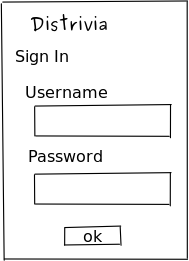
\includegraphics[scale=0.3]{design-pictures/login.png}
  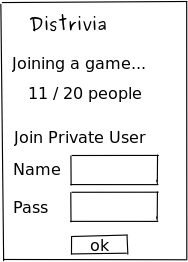
\includegraphics[scale=0.3]{design-pictures/joingame.png}
  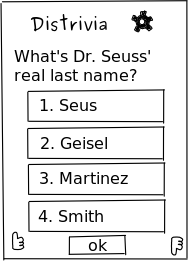
\includegraphics[scale=0.3]{design-pictures/quiz.png}
  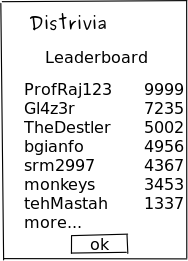
\includegraphics[scale=0.3]{design-pictures/leaderboard.png}


\subsection{Backend}
The server has four key layers involved.
First, there will be load balancer that accepts all messages from the players.
It does not need to read the contents of the message, it simply distributes the message on to the most reliable server with the lowest load.
This ensures that if any of the servers were to go down, that the system would still run.
It also maintains highest speeds for server response.
The message is passed to a web server from the load balancer, which will read the contents of the message and respond appropriately.
These messages will be in the form of http messages.
The web server communicates directly with the database to perform whatever actions need to be done.
The third layer is represented by these synchronous databases that hold all the actual data for the software.
This would include round information, player information, and all the questions for the application.
The fourth and final layer would be some sort of master process that does the actual synchronization between the databases so that they all contain repetitive data for reliable communication.

\begin{center}
  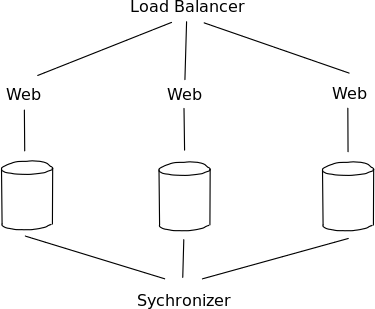
\includegraphics[scale=0.3]{design-pictures/database.png}
\end{center}

\newpage
%
% The following two commands are all you need in the
% initial runs of your .tex file to
% produce the bibliography for the citations in your paper.
%/\bibliographystyle{abbrv}
%\bibliography{bibliography}  % sigproc.bib is the name of the Bibliography in this case
% You must have a proper ".bib" file
%  and remember to run:
% latex bibtex latex
% to resolve all references
%
% ACM needs 'a single self-contained file'!
%
%APPENDICES are optional
\balancecolumns
% That's all folks!
\end{document}
